\documentclass[10pt,twocolumn]{article}

% use the oxycomps style file
\usepackage{oxycomps}

% usage: \fixme[comments describing issue]{text to be fixed}
% define \fixme as not doing anything special
\newcommand{\fixme}[2][]{#2}
% overwrite it so it shows up as red
\renewcommand{\fixme}[2][]{\textcolor{red}{#2}}
% overwrite it again so related text shows as footnotes
%\renewcommand{\fixme}[2][]{\textcolor{red}{#2\footnote{#1}}}

% read references.bib for the bibtex data
\bibliography{references}

% include metadata in the generated pdf file
\pdfinfo{
    /Title (Autonomous Vehicle - Final Paper)
    /Author (James Derrod)
}

% set the title and author information
\title{Autonomous Vehicle - Final Paper}
\author{James Derrod}
\affiliation{Occidental College}
\email{jderrod@oxy.edu}

\begin{document}

\maketitle

\section{Problem Statement}

This project addresses the challenge of developing and testing autonomous driving systems through simulation-based reinforcement learning. This autonomous driving problem requires an agent to control a car to navigate randomly generated racetracks while making real-time decisions about steering, acceleration, and braking, given input about their environment. The agent aims to develop a policy which can maximize the reward it earns within an episode. To address this challenge, a 2D simulated environment was used which creates a controlled testing ground where an agent can safely learn driving behaviors through trial and error, without the high costs and safety risks associated with real-world vehicle testing.
    
Autonomous driving technology has the potential to significantly improve transportation safety and accessibility. The World Health Organization reports that approximately 1.2 million people die each year from road traffic accidents\cite{WHORoadTraffic}, human error being a major contributing factor. By developing more sophisticated autonomous driving systems, we can work towards reducing these accidents. Furthermore, simulation-based training environments open up the possibility of democratizing autonomous vehicle research, allowing more researchers and institutions to contribute to the advancement of this technology.

Value proposition: using reinforcement learning for complex driving tasks


\section{Technical Background}
Reinforcement learning, vehicle physics simulation, and procedural track generation form the foundation of this autonomous driving project. Each component plays a vital role in creating an environment where an AI agent can learn to navigate racing tracks efficiently.

\subsection{Reinforcement Learning and Markov Decision Process}
Reinforcement learning operates on the principle of learning through interaction and feedback, mathematically formalized through a Markov Decision Process (MDP)\cite{MarkovDecisionProcess}. This framework breaks down complex tasks like autonomous driving into components that a computer can process and learn from:
\begin{itemize}
\item Agent and Environment: The agent (controlling the car) interacts with the environment (the race track) by observing its state and taking actions.
    \item State Space (\textbf{S}): Represents what the agent can observe about its environment. In the driving scenario, this includes the car's speed, position on the track, distance from track boundaries, and information about upcoming turns.

    \item Action Space (\textbf{A}): Describes the possible actions an agent can take. The car has three continuous actions: steering (turning left or right), acceleration (speeding up), and braking (slowing down), each applicable with varying intensity.

    \item Transition Function (\textbf{P}): Defines how actions change the current state. In a physics-based environment, this represents how the car's position and speed change when the agent applies controls. This is handled by Unity's physics system.

    \item Reward Function (\textbf{R}): Provides feedback on the agent's performance. The agent receives positive rewards for staying on track and progressing or completing laps, while receiving penalties for actions like hitting track boundaries or driving inefficiently.
\end{itemize}

Unlike traditional rule-based programming, this framework enables the agent to discover optimal driving strategies through trial and error. The agent develops a policy, otherwise known as a strategy for choosing actions by maximizing its cumulative rewards over time. This approach allows the agent to learn complex behaviors without explicitly programming rules for every possible situation.

\subsection{Proximal Policy Optimization (PPO)}
Proximal Policy Optimization (PPO) is the reinforcement learning algorithm used in this project. PPO improves upon traditional policy gradient methods by implementing a clipped objective function that prevents large policy updates, which can destabilize training\cite{schulman2017proximal}. The algorithm works by:

\begin{itemize}
    \item Collecting data from the current policy as the agent interacts with the environment
    \item Computing the ratio between new and old policies
    \item Clipping this ratio to limit the size of policy updates
    \item Optimizing a surrogate objective function that balances exploration and exploitation
\end{itemize}

This approach makes PPO particularly suitable for continuous control tasks like autonomous driving, as it provides stable learning while being computationally efficient. The algorithm's conservative update strategy helps prevent catastrophic performance drops during training, which is crucial when learning complex driving behaviors.

\subsection{Vehicle Physics in 2D}
This project implements a 2D vehicle physics model that captures key driving dynamics:
\begin{itemize}
    \item Forward Force: Acceleration in the direction the car is facing.
    \item Turning Force: Rotation of the car based on steering input.
    \item Friction: Resistance to movement that affects the car's ability to turn (drift).
    \item Momentum: The car's tendency to keep moving in its current direction.
\end{itemize}


These physics elements provide realistic vehicle behavior while maintaining computational efficiency, creating a balance between accuracy and learning performance.

\subsection{Procedural Track Generation}
Procedural track generation is based on spline mathematics, a fundamental concept in computational geometry. Splines are piecewise polynomial functions that create smooth curves by interpolating between control points. The key mathematical components include:
\begin{itemize}
    \item Bézier curves: Mathematical curves governed by control points that define their shape and curvature
    \item Interpolation: The process of creating continuous curves between discrete points while maintaining smoothness
    \item Tangent Vectors: Directional guides at control points that influence curve smoothness and shape
\end{itemize}
In the context of race track generation, these mathematical principles ensure:
\begin{itemize}
    \item Continuous curvature between track segments
    \item Physical feasibility of the racing surface
    \item Controllable geometric properties (such as minimum turn radius)
\end{itemize}

Understanding these foundations is crucial because they determine the way in which the agent is trained, as well as the drivability of the generated tracks, and directly impact the learning environment's quality for autonomous agents.

\section{Prior Work}
Research in autonomous driving and reinforcement learning can be grouped into three main areas that inform this project: commercial autonomous driving systems, reinforcement learning in vehicle control, and simulation-based training approaches.
\subsection{Commercial Autonomous Systems}
Tesla's development of Autopilot and Full Self-Driving (FSD) systems demonstrates the practical challenges of autonomous driving. While Tesla primarily uses supervised learning and computer vision approaches rather than reinforcement learning, their work highlights the importance of extensive testing and iterative development in controlled environments before deployment. This aligns with the project's simulation-first approach to autonomous vehicle development.
\subsection{Reinforcement Learning in Vehicle Control}
Recent advances in reinforcement learning for vehicle control have established several key approaches:
\begin{itemize}
    \item Deep Q-Networks (DQN) have shown promise in vehicle control tasks, particularly for discrete action spaces. Wang et al. demonstrated that DQN-based systems can effectively handle complex driving scenarios while maintaining computational efficiency \cite{10492530}. This project builds upon this work by extending these principles to continuous action spaces.
\   item Kiran et al. conducted a comprehensive survey of deep reinforcement learning in autonomous driving, establishing a taxonomy of driving tasks and their corresponding algorithmic approaches            \cite{9351818}. Their work informed the choice of PPO (Proximal Policy Optimization) algorithm and state space design.

\item Wang et al.'s research on highway driving scenarios showed how reinforcement learning can handle high-speed decision-making tasks \cite{9190040}. While this project focuses on racing scenarios rather than highway driving, we adopt similar principles for handling high-speed navigation and trajectory planning.
\end{itemize}
\subsection{Simulation-Based Training}
Simulation environments have become increasingly important in autonomous vehicle development, offering several advantages over real-world training:
\begin{itemize}
\item Safety: Allows for exploration of dangerous scenarios without real-world risk
\item Speed: Enables rapid iteration and testing of different approaches
\item Cost: Eliminates the need for expensive physical prototypes during initial development
\end{itemize}
This project builds upon these previous works while focusing specifically on the challenge of autonomous racing through reinforcement learning in a customized Unity simulation environment. This approach allows us to combine the benefits of simulation-based training with the adaptability of reinforcement learning algorithms.

\section{Methods}

\subsection{Track Generation System}
The track generation system employs Unity's spline system for creating varied racing environments. The system generates tracks using three primary components: spline-based path generation, turn placement, and difficulty adjustment.
The base track is constructed using a configurable number of control points (default=25) arranged in a circular pattern. Each control point influences the shape of the track through Bézier curve interpolation, ensuring smooth transitions between track segments. Track width is maintained as a constant parameter throughout the course, defining the drivable area's boundaries.

The turn system introduces complexity through three key parameters:
\begin{itemize}
    \item Starting Turns: Initial number of turns (default=3)
    \item Maximum Turns: Upper limit for turn count (default=6)
    \item Turn Intensity: Controls turn sharpness (default=3.0)
\end{itemize}

Turns are placed along the track with enforced minimum spacing to prevent impossible sequences. Each turn modifies the base circular path by adjusting control points, creating natural deviations in the track's curvature.
The difficulty progression system adapts track complexity based on agent performance. After each training episode, the system records whether the agent successfully completed the track. When the agent achieves a 75\% completion rate over the last 100 episodes, the system increases track complexity by adding additional turns, up to the maximum limit. This adaptive approach ensures the agent faces increasingly challenging scenarios only after demonstrating competence at the current difficulty level.

\includegraphics[scale=.75]{track}
\caption{Image of a randomly generated track.}
\label{fig:track}

\subsection{Agent Design}
The autonomous racing agent integrates sensor data, state observations, continuous actions, and a structured reward system to learn optimal racing behavior.

\subsubsection{Sensor System}
The agent perceives its environment through five raycasts positioned strategically around the vehicle: two side-facing rays for lateral distance detection, two 45-degree forward-angled rays for upcoming obstacle detection, and one forward-facing ray. Each raycast returns a normalized distance value between 0 and 1, representing the distance to track boundaries. This design provides the agent with essential proximity information while maintaining computational efficiency.

\subsubsection{State Observation Space}
The agent's observation space combines multiple data streams to provide comprehensive track awareness:
\begin{itemize}
    \item Vehicle dynamics: Current velocity (x, y components), angular velocity, and time since last checkpoint
    \item Track progress: Distance to next checkpoint, current progress along spline (normalized position)
    \item Forward planning: Five look-ahead points on the track, providing advance information about upcoming track segments
    \item Turn information: Distance and direction to the next turn point, enabling anticipation of challenging track sections
\end{itemize}

\subsubsection{Action Space}
The agent operates with a continuous action space consisting of three parameters:
\begin{itemize}
    \item Steering: Continuous value between -1 (full left) and 1 (full right)
    \item Acceleration: Continuous value between 0 and 1 (no acceleration -> full acceleration)
    \item Braking: Continuous value between 0 and 1 (no braking power -> full braking power)
\end{itemize}
These actions interact with Unity's physics system to produce realistic vehicle behavior, including momentum and drift effects.

\subsubsection{Reward Structure}
The reward system encourages both progression and skillful driving:
Progressive Rewards:
\begin{itemize}
    \item +1 for reaching each new spline point
    \item +3 for successfully completing a turn
    \item +10 for completing a full lap
\end{itemize}
Penalties:
\begin{itemize}
    \item -5 for collision with track boundaries
    \item -8 for timeout (failing to progress)
\end{itemize}
This reward structure was designed to prioritize continuous forward progress while encouraging the completion of challenging track segments. The higher penalty for timeouts compared to collisions ensures the agent maintains forward momentum rather than becoming overly cautious.

\subsection{Training Implementation}
\subsubsection{PPO Configuration}
The agent was trained using Proximal Policy Optimization (PPO) with the following architecture and parameters:
Network Configuration:
\begin{itemize}
    \item Two hidden layers with 256 units each
    \item Normalized input and hidden states
    \item Simple visual encoding type
\end{itemize}
Key Hyperparameters:
\begin{itemize}
    \item Batch size: 2048
    \item Buffer size: 20480
    \item Learning rate: 0.0003 (linear schedule)
    \item Gamma (discount factor): 0.99
    \item Lambda: 0.95
    \item Number of epochs: 4
\end{itemize}
Each training session ran for approximately 20-24 hours, accumulating 5-15 million steps per run.
\subsubsection{Curriculum Learning}
The training process implemented a performance-based curriculum:
\begin{itemize}
    \item Evaluation Window: Performance measured over 100 episodes
    \item Success Threshold: 75\% lap completion rate required for difficulty increase
    \item Progression: Incrementally increased track complexity through turn count and intensity
\end{itemize}

\subsubsection{Evolution of Training Approach}
The training process evolved through three major iterations:
First Iteration:
\begin{itemize}
    \item Basic reward structure focused on checkpoint completion
    \item Agent achieved sporadic success on simple tracks with three turns
    \item Identified need for more structured rewards
\end{itemize}
Second Iteration:
\begin{itemize}
    \item Added lap completion rewards
    \item Achieved significantly higher mean rewards
    \item Agent demonstrated ability to complete multiple consecutive laps
\end{itemize}
Third Iteration:
\begin{itemize}
    \item Introduced turn-specific rewards and observations
    \item Implemented adaptive difficulty progression
    \item Encountered challenges with increased complexity, suggesting potential oversaturation of the observation space or need for hyperparameter adjustment
\end{itemize}
Each iteration provided insights that informed subsequent training approaches, though the increased complexity in the final iteration revealed potential limitations in the current architecture that warrant further investigation.


\section{Evaluation Metrics}
The mean reward per episode served as the primary quantitative measure, reflecting the agent's overall effectiveness in completing track objectives. During successful training runs, mean rewards reached into the hundreds, indicating multiple checkpoint completions and successful lap navigation.

Episode length, measured in steps, provided insight into the agent's efficiency and consistency. Longer episodes typically indicated successful navigation, while shorter episodes often resulted from early collisions or timeout failures. Successful agents maintained episode lengths sufficient to complete multiple laps, approximately 500-1000 steps per lap depending on track complexity.

The lap completion rate proved particularly valuable for assessing agent reliability. This metric tracked the percentage of episodes where the agent successfully completed a full circuit of the track. In the most successful iteration (second training run), the agent achieved consistent lap completions, maintaining the required 75\% success rate over 100-episode windows.

Turn completion success rate, introduced in the third iteration, specifically measured the agent's ability to navigate challenging track segments. Each successful turn completion earned a +3 reward, allowing us to track the agent's proficiency at handling these critical track features.

\subsubsection{Training Progress Metrics}
We monitored training progress through TensorBoard, tracking reward trends and learning stability. Key indicators included:
\begin{itemize}
    \item Running average of episode rewards
    \item Frequency of successful lap completions
    \item Distribution of episode lengths
    \item Rate of premature episode terminations
\end{itemize}
These metrics revealed clear patterns in the agent's learning progression, including both steady improvements and plateau periods where performance stabilized or occasionally degraded.



\subsection{Comparative Analysis}
\subsubsection{Across Training Iterations}
The agent's capabilities evolved significantly across three training iterations:
\begin{itemize}
    \item First Iteration:
    \begin{itemize}
        \item Achieved basic track navigation with sporadic success on tracks with three turns
        \item Mean rewards remained relatively low, indicating inconsistent performance
        \item Limited ability to handle track variations or complete full laps consistently
    \end{itemize}
    \item Second Iteration:
    \begin{itemize}
        \item Introduced lap completion rewards (+10), leading to dramatically improved performance
        \item Mean rewards reached hundreds, indicating multiple lap completions
        \item Demonstrated consistent ability to navigate tracks with 3-4 turns
        \item Showed marked improvement in maintaining continuous forward progress
    \end{itemize}
    \item Third Iteration:
    \begin{itemize}
        \item Added turn awareness and adaptive difficulty
        \item Initially showed promise with turn-specific learning
        \item Performance plateaued when facing increased complexity
        \item Suggested possible limitations in the current architecture when handling multiple objectives
    \end{itemize}
\end{itemize}


\subsubsection{Performance at Different Difficulty Levels}
Track difficulty variations revealed clear performance patterns:
\begin{itemize}
\item Turn Count Impact: Performance decreased notably as turns increased from 3 to 6
\item Turn Intensity: Higher turn intensity (>3.0) significantly reduced completion rates
\item Track Width: Wider tracks generally resulted in higher completion rates
\end{itemize}
\subsection{Failure Analysis}
\subsubsection{Common Failure Modes}
Analysis of unsuccessful episodes revealed several recurring patterns:
Timeout Scenarios:
\begin{itemize}
    \item Most common in complex track sections with multiple consecutive turns
    \item Often occurred when the agent became "stuck" trying to navigate tight turns
    \item Indicated potential issues with the agent's long-term planning capabilities
\end{itemize}

Collision Patterns:
\begin{itemize}
    \item Frequently occurred at turn entry points
    \item More common with higher turn intensity settings
    \item Often resulted from excessive speed entering turns
\end{itemize}

Training Plateaus:
\begin{itemize}
    \item Occurred consistently when complexity increased too rapidly
    \item Suggested limitations in the agent's ability to handle multiple objectives simultaneously
    \item Indicated potential issues with the reward structure balancing
\end{itemize}

\subsubsection{Performance Limitations}
Analysis revealed several key limitations:
Complexity Threshold:
\begin{itemize}
    \item Agent performance degraded significantly beyond 4 turns per track
    \item Struggled to maintain consistent performance when multiple learning objectives were introduced
    \item Showed difficulty generalizing to more complex track layouts
\end{itemize}

Behavioral Inconsistencies:
\begin{itemize}
    \item Occasional erratic behavior even after successful training
    \item Some inconsistent performance across similar track configurations.
\end{itemize}


Training Stability:
\begin{itemize}
    \item Third iteration showed signs of catastrophic forgetting.
    \item Increased complexity led to unstable learning patterns.
\end{itemize}

These limitations point to several areas for future improvement, particularly in the agent's ability to handle increased track complexity while maintaining stable performance.


\section{Results and Discussion}
Evaluation of autonomous racing agent across multiple training iterations revealed both significant achievements and notable limitations in reinforcement learning for autonomous racing. The findings span three key areas:
\subsection{Training Performance Analysis}
\subsubsection{Learning Progression}
\begin{itemize}
\item Reward accumulation showed distinct patterns across iterations, with initial slow progress followed by periods of rapid improvement
\item First iteration achieved basic navigation but with inconsistent rewards, rarely exceeding single-lap completion

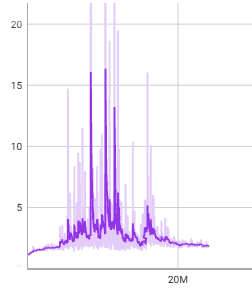
\includegraphics[scale=.75]{run1}
\caption{Mean reward per episode during the first training iteration. The graph shows sporadic success in basic track navigation with relatively low and inconsistent rewards.}
\label{fig:run1-mean-reward}

\item Second iteration demonstrated significant improvement, with mean rewards reaching hundreds, indicating multiple lap completions]


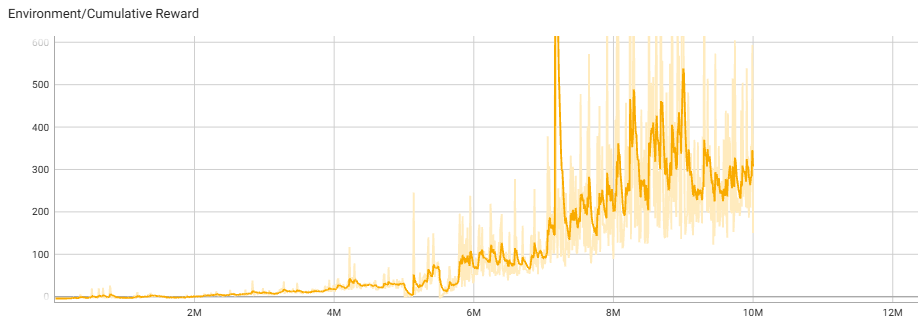
\includegraphics[scale=.4]{run2}
\caption{Mean reward per episode during the first training iteration. The graph shows sporadic success in basic track navigation with relatively low and inconsistent rewards.}
\label{fig:run2-mean-reward}

\item Third iteration initially showed promise but struggled with the increased complexity of turn-specific objectives
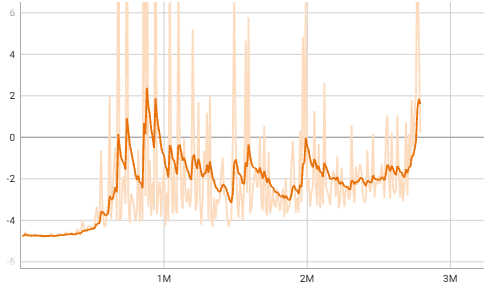
\includegraphics[scale=.75]{run3}
\caption{Mean reward per episode during the first training iteration. The graph shows sporadic success in basic track navigation with relatively low and inconsistent rewards.}
\label{fig:run3-mean-reward}

\end{itemize}
\subsubsection{Behavioral Analysis}
\begin{itemize}
\item Agent developed efficient navigation strategies for straightaways and basic turns
\item Learning emerged in stages: first maintaining track position, then optimizing speed, and finally attempting turn optimization
\item Vehicle control became more refined over time, with smoother acceleration and braking patterns
\item Turn handling showed adaptation to different angles and intensities, though performance decreased with turn complexity
\end{itemize}
\subsection{Performance Benchmarks}
\subsubsection{Track Navigation}
\begin{itemize}
\item Second iteration achieved the best results, demonstrating consistent multi-lap completions
\end{itemize}
\subsection{System Limitations and Challenges}
\subsubsection{Technical Constraints}
\begin{itemize}
\item Training sessions were quite long.
\item Five-raycast sensor system showed limitations in complex scenarios
\item Training required 5-15 million steps per iteration to achieve stable performance
\end{itemize}
\subsubsection{Learning Challenges}
\begin{itemize}
\item Performance degraded significantly with tracks containing more than 4 turns
\item Agent struggled to balance multiple objectives when turn-specific rewards were introduced
\item Difficulty generalizing learned behaviors to substantially different track layouts
\item Evidence of catastrophic forgetting during third iteration when complexity increased
\end{itemize}
\subsection{Future Improvements}
\subsubsection{Architectural Enhancements}
\begin{itemize}
\item Implement additional sensor rays for better environmental awareness
\item Explore deeper neural network architectures to handle increased complexity
\item Investigate alternative PPO configurations to improve training stability, or alternative learning algorithms.
\item Consider implementing a memory system to better handle long-term dependencies
\end{itemize}
\subsubsection{Training Refinements}
\begin{itemize}
\item Develop more granular curriculum learning stages
\item Implement dynamic reward scaling based on task difficulty
\item Explore transfer learning to preserve successful behaviors while learning new skills
\item Consider implementing a hybrid reward system that better balances multiple objectives
\end{itemize}
These results demonstrate that while reinforcement learning can successfully teach an agent basic autonomous racing skills, significant challenges exist in scaling to more complex scenarios. The success of the second iteration suggests that carefully balanced reward structures and appropriate complexity progression are crucial for effective learning.

\section{Ethical Considerations}
The development of autonomous racing systems raises key ethical considerations that extend beyond simulation to real-world applications. This project addresses these concerns in two main areas:
\begin{itemize}
\item \textbf{Safety in Development}: Simulation-based training provides a risk-free environment for testing autonomous driving behaviors that would be dangerous to explore with physical vehicles. This approach allows for extensive testing of edge cases and aggressive maneuvers without endangering people or property.
\item \textbf{System Transparency}: Reinforcement learning agents can develop effective but difficult-to-interpret decision-making processes. By documenting the agent's success and failure modes\cite{AVPowerInequity}, we contribute to understanding reinforcement learning limitations in autonomous systems and highlight areas where improved transparency is needed.
\end{itemize}
Future work should focus on incorporating explicit safety constraints and developing more interpretable decision-making processes\cite{AlgorithmBiasInAutonomousSystems} to ensure that advances in autonomous vehicles maintain safety as a priority.

\section{Replication Instructions}
To replicate this project, go to https://github.com/jderrod/JamesDerrodCompsProjectCode and clone the repository. Open up in unity, and go to the "project" scene. 

To run, ensure the car agent script attatched to the car is in default mode, not heuristic or inference. Insert the trained model by dropping in the .onnx file from the results folder "1" or "5". Choose the .onnx file with the highest number and run the program. To train headlessly,  running within the directory:

Start the virtual environment with: "MLvenv\Scripts\activate", then,
"mlagents-learn Assets/training_config.yaml --env="Builds/Comps Project 2.exe" --run-id=new_run_id --no-graphics"

\section{Code Architecture Overview}
This autonomous racing system consists of two primary components: the TrackGenerator and CarAgent classes, which handle environment generation and agent behavior respectively.
\subsection{TrackGenerator Class}
The track generation system manages procedural track creation and difficulty progression:
\begin{itemize}
\item \textbf{Track Creation Pipeline}:
\begin{itemize}
\item GenerateRandomSpline(): Creates base track shape
\item GenerateTrackMesh(): Converts spline to drivable surface
\item PlaceTurnMarkers(): Handles turn point identification
\end{itemize}
Copy\item \textbf{Difficulty Management}:
\begin{itemize}
    \item RecordLapCompletion(): Tracks agent performance
    \item GenerateRandomTurnIndices(): Controls turn placement
    \item Dynamic difficulty adjustment based on completion rates
\end{itemize}
\end{itemize}
\subsection{CarAgent Class}
The agent implementation extends Unity's ML-Agents framework:
\begin{itemize}
\item \textbf{Core Components}:
\begin{itemize}
\item CollectObservations(): Gathers environment state
\item OnActionReceived(): Processes agent decisions
\item GetTrackEdgeSensorReadings(): Manages sensor system
\end{itemize}
Copy\item \textbf{Physics Integration}:
\begin{itemize}
    \item ApplyCarControls(): Handles vehicle physics
    \item IsWithinTrackBounds(): Manages boundary detection
    \item CheckProgressTimer(): Tracks agent progress
\end{itemize}
\end{itemize}
Extension points for future development include:
\begin{itemize}
\item Additional sensor types in GetTrackEdgeSensorReadings()
\item New reward mechanisms in CheckProgressTimer()
\item Enhanced track generation features in GenerateRandomSpline()
\item Extended difficulty progression logic in RecordLapCompletion()
\end{itemize}
\printbibliography

\end{document}


